\documentclass[margin=5mm]{standalone}
\usepackage[dvipsnames]{xcolor}
\usepackage{pgfplots}
\usepackage{tikz}
\usepackage[tikz]{ocgx2}

\pgfplotsset{compat=1.18}
\begin{document}

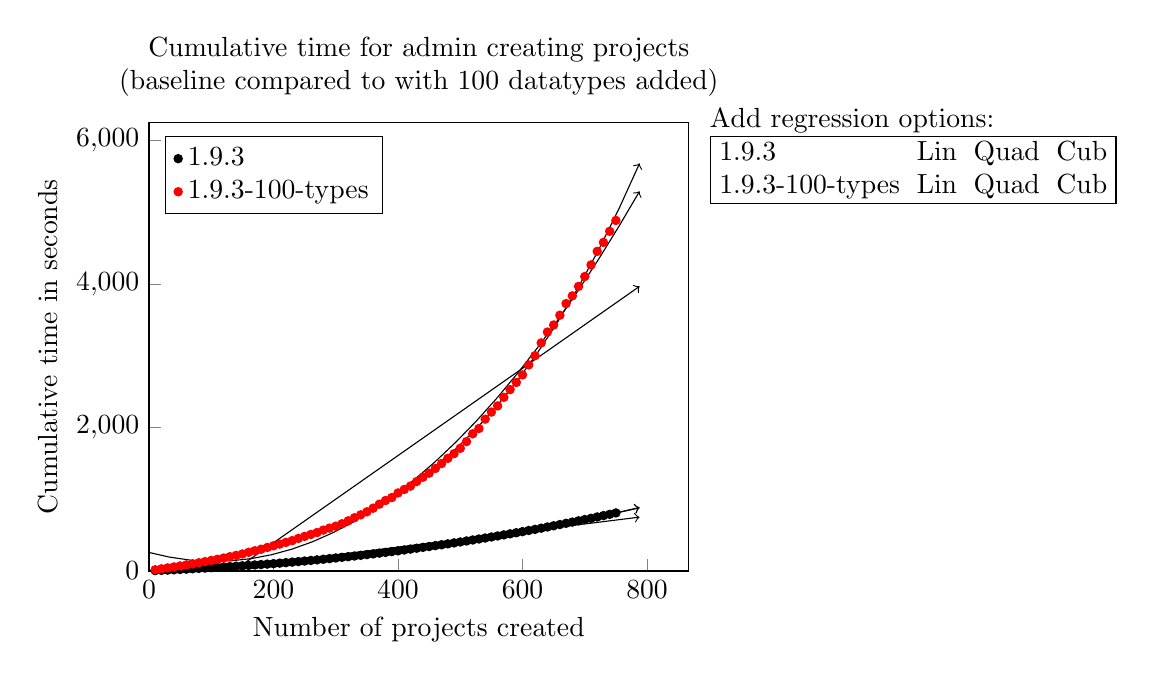
\begin{tikzpicture}
    \begin{axis}[
        align = center,
        legend pos = north west,
        legend cell align = left,
        xlabel = Number of projects created,
        ylabel = Cumulative time in seconds,
        xtick pos = left,
        ytick pos = left,
        scaled ticks = false,
        xmin = 0,
        ymin = 0,
        title = {Cumulative time for admin creating projects (baseline compared to with 100 datatypes added)},
        title style = {text width = 0.8\textwidth},
        legend entries={\switchocg{1.9.3}{1.9.3},\switchocg{1.9.3-100-types}{1.9.3-100-types}}]
        \begin{scope}[ocg = {ref = 1.9.3-Lin, status = invisible}]
            \plot[domain=0:788,->,forget plot] (\x,{-98.54166666666651508421637117862701416015625 + 1.0772444210526312957654226920567452907562255859375*(\x)^1});
        \end{scope}
        \begin{scope}[ocg = {ref = 1.9.3-Quad, status = invisible}]
            \plot[domain=0:788,->,forget plot] (\x,{7.32380325805269105643446891917847096920013427734375 + 0.2523186813794946470324020992848090827465057373046875*(\x)^1 + 0.00108542860483307472725666986690384874236769974231719970703125*(\x)^2});
        \end{scope}
        \begin{scope}[ocg = {ref = 1.9.3-Cub, status = invisible}]
            \plot[domain=0:788,->,forget plot] (\x,{4.302698042700395575366201228462159633636474609375 + 0.298498061886172172396669566296623088419437408447265625*(\x)^1 + 0.00093452424842187134350346422451139005715958774089813232421875*(\x)^2 + 0.000000132372242465967984971240219323196374290318999555893242359161376953125*(\x)^3});
        \end{scope}
        \begin{scope}[ocg = {ref = 1.9.3, status = visible}]
            \addplot[
                only marks,
                color = black,
                mark = *,
                mark size = 1.5 pt
            ]coordinates {(10,4.893)(20,8.565)(30,12.45)(40,16.481)(50,20.969)(60,25.598)(70,30.393)(80,35.513)(90,40.692)(100,46.193)(110,50.884)(120,55.874)(130,61.273)(140,66.624)(150,72.007)(160,77.52)(170,83.484)(180,89.332)(190,95.407)(200,101.951)(210,109.26)(220,116.023)(230,123.257)(240,130.729)(250,138.308)(260,146.558)(270,154.832)(280,162.92)(290,172.04)(300,180.864)(310,190.073)(320,199.053)(330,208.464)(340,217.838)(350,227.782)(360,237.676)(370,248.49)(380,259.002)(390,269.871)(400,280.599)(410,292.408)(420,304.925)(430,316.866)(440,328.832)(450,340.744)(460,353.117)(470,365.289)(480,377.698)(490,391.141)(500,404.275)(510,417.943)(520,431.625)(530,445.695)(540,459.277)(550,473.455)(560,487.956)(570,502.917)(580,517.465)(590,532.707)(600,548.142)(610,564.148)(620,579.597)(630,596.346)(640,613.199)(650,630.032)(660,647.052)(670,664.296)(680,681.433)(690,699.036)(700,716.467)(710,734.169)(720,752.817)(730,771.651)(740,789.499)(750,808.88)};
        \end{scope}
        \begin{scope}[ocg = {ref = 1.9.3-100-types-Lin, status = invisible}]
            \plot[domain=0:788,->,forget plot] (\x,{-822.945556036036578007042407989501953125 + 6.079636586059745440024926210753619670867919921875*(\x)^1});
        \end{scope}
        \begin{scope}[ocg = {ref = 1.9.3-100-types-Quad, status = invisible}]
            \plot[domain=0:788,->,forget plot] (\x,{258.04641898555888701594085432589054107666015625 + -2.343677505017625950500814724364317953586578369140625*(\x)^1 + 0.01108330801457549190380813541878524119965732097625732421875*(\x)^2});
        \end{scope}
        \begin{scope}[ocg = {ref = 1.9.3-100-types-Cub, status = invisible}]
            \plot[domain=0:788,->,forget plot] (\x,{-6.86636237525271386772374171414412558078765869140625 + 1.7056710808497097531244435231201350688934326171875*(\x)^1 + -0.0021490986468037701594135935323492958559654653072357177734375*(\x)^2 + 0.000011607374264367779012076774269868195688104606233537197113037109375*(\x)^3});
        \end{scope}
        \begin{scope}[ocg = {ref = 1.9.3-100-types, status = visible}]
            \addplot[
                only marks,
                color = red,
                mark = *,
                mark size = 1.5 pt
            ]coordinates {(10,16.646)(20,29.422)(30,42.437)(40,56.08)(50,70.139)(60,84.764)(70,98.978)(80,114.168)(90,129.882)(100,146.828)(110,162.99)(120,180.553)(130,199.315)(140,217.459)(150,236.641)(160,260.138)(170,281.308)(180,302.897)(190,327.593)(200,350.446)(210,374.874)(220,398.411)(230,422.911)(240,453.814)(250,482.088)(260,508.805)(270,535.495)(280,569.978)(290,597.273)(300,624.35)(310,658.328)(320,698.895)(330,741.721)(340,782.599)(350,824.435)(360,875.311)(370,930.797)(380,982.759)(390,1023.689)(400,1087.313)(410,1135.987)(420,1182.763)(430,1246.736)(440,1306.875)(450,1363.422)(460,1429.908)(470,1497.549)(480,1570.16)(490,1635.807)(500,1710.053)(510,1803.519)(520,1912.432)(530,1986.123)(540,2116.806)(550,2215.404)(560,2301.122)(570,2420.667)(580,2528.409)(590,2628.704)(600,2734.008)(610,2873.265)(620,3001.612)(630,3179.378)(640,3330.69)(650,3429.12)(660,3565.541)(670,3727.599)(680,3835.233)(690,3966.829)(700,4105.051)(710,4267.078)(720,4455.357)(730,4581.11)(740,4735.104)(750,4886.775)};
        \end{scope}
    \end{axis}
    \begin{scope}
        \addtolength{\tabcolsep}{-0.3em}
        \node [below right, shape=rectangle, align=left](regressiontable) at (7,6) {
            Add regression options: \\
            \begin{tabular}{|llll|}
                \hline
                1.9.3 & \switchocg{1.9.3-Lin}{Lin} & \switchocg{1.9.3-Quad}{Quad} & \switchocg{1.9.3-Cub}{Cub} \\
                1.9.3-100-types & \switchocg{1.9.3-100-types-Lin}{Lin} & \switchocg{1.9.3-100-types-Quad}{Quad} & \switchocg{1.9.3-100-types-Cub}{Cub} \\
                \hline
            \end{tabular}
        };
    \end{scope}
\end{tikzpicture}

\end{document}